\documentclass[a4 paper, 12pt]{article}
\usepackage[slovene]{babel}
\usepackage[utf8]{inputenc}
\usepackage[T1]{fontenc}
\usepackage[small, width=0.9\textwidth,labelfont=it]{caption}
\usepackage[pdftex]{graphicx}
\usepackage{amssymb, fullpage, float, pdflscape, subcaption, amsmath, color, hyperref}

\renewcommand{\d}{
	\ensuremath{\mathrm{d}}
}

\newcommand{\e}{
	\ensuremath{\mathrm{e}}
}

\renewcommand{\r}{
	\ensuremath{\mathbf{r}}
}

\begin{document}

\begin{center}
\textsc{Modelska analiza II}\\
\textsc{2011/12}\\[0.5cm]
\textbf{7. naloga -- Metoda kon\v cnih elementov: Poissonova ena\v cba}
\end{center}
\begin{flushright}
\textbf{Jože Zobec}\\
\end{flushright}

\section{Uvod}

Spet se vra\v camo k Poissonovi ena\v cbi. Merimo hitrostni profil skozi cev, katere profil je
lik (mnogoterost) $\mathcal{A}$. V brezdim. obliki se ena\v cba zapi\v se kot
\begin{equation}
	\nabla^2 v = -f,
	\label{poisson}
\end{equation}
robni pogoj pa je $v(\partial \mathcal{A}) = 0$. Prostor diskretiziramo tako, da ga najprej
tlakujemo s poljubnimi liki. Najprikladnej\v si so trikotniki, saj lahko z njmi relativno
natan\v cno opi\v semo vsako obliko. Za to je posebej prikladna Delaunayeva triangulacija, ki
ima implementacije v raznoterih knji\v znicah in programih.

Po triangulaciji aproksimiramo $\mathcal{A} \approx \mathcal{A'}$, katero sestavlja $N$ vozli\v s\v c
in $M$ trikotnikov. Dokazano je, da ena\v cbo~\eqref{poisson} re\v simo (dobimo $v$) natanko tedaj,
poi\v s\v cemo tak $A(w, v)$, da
\begin{equation}
	\sum_{t = 1}^M A^{(t)}(w, v) = \sum_{t = 1}^M \langle w, f \rangle^{(t)},
\end{equation}
kjer $t$ predstavlja indeks po trikotnikih, $A(w,v)^{(t)}$ in $\langle w, f\rangle^{(t)}$ pa sta
\begin{equation}
	A (w, v)^{(t)} = \int_{T_t} \big[(\nabla w)^T \cdot (\nabla v) + wv\big]\ \d x~\d y,\quad
	\langle w, f\rangle^{(t)} = \int_{T_t} w f\ \d x~\d y.
	\label{crap-pap}
\end{equation}
Funkcija $w$ je ute\v zna funkcija. Tako $v$, kot $w$ aproksimiramo z razvojem po baznih funkcijah
\begin{equation}
	v \approx \sum_{j = 1}^N c_j \phi_j (x, y),\quad w \approx \sum_{j = 1} d_j \psi_j (x, y),
\end{equation}
vendar bomo vzeli Galerkinov na\v cin in rekli $\psi_j = \phi_j$. Te funkcije izgledajo kot
Trikotnik $T_t$ imenujemo kon\v cni element. Vsak trikotnik ima notranje indkse, $m$, $n$, ki
te\v cejo po ogli\v s\v cih trikotnika. Nad trikotnikom z ogli\v s\v ci $\r_1^j = (x_1, y_1)^T$,
$\r_2^j = (x_2, y_2)^T$ in $\r_3^j = (x_3, y_3)^T$, kjer funkcija $\phi_j (x,y)$ zapi\v se kot
\begin{equation}
	\phi_j (x,y) = \left[\det \begin{pmatrix}
			1 & x_1^j & y_1^j \\
			1 & x_2^j & y_2^j \\
			1 & x_3^j & y_3^j
		\end{pmatrix} \right]^{-1} \det \begin{pmatrix}
			1 & x     & y     \\
			1 & x_2^j & y_2^j \\
			1 & x_3^j & y_3^j
		\end{pmatrix},
\end{equation}
o\v citno je, da je $\r_1^j$ kar enak vozli\v s\v cu $\r_j$. Funkcija $\phi_j (x,y)$ ni definirana samo
nad trikotnikom, ampak nad vsemi sosedi vozli\v s\v ca $\r_j$ (tj. nad vsemi trikotniki, katerih
ogli\v s\v ce je $\r_j$). Velja tudi $\phi_j (\r_k) = \delta_{j,k}$. V ena\v cbi~\eqref{crap-pap}
potrebujemo gradiente: $\nabla \phi_j$, ki so
\begin{equation}
	\nabla \phi_j = \frac{1}{2|T|} \begin{pmatrix} y^j_2 - y^j_3 \\ x^j_3 - x^j_2 \end{pmatrix}.
\end{equation}
Lokalne prispevke znotraj trikotnika $t$ lahko potem z indeksoma $m$, $n$, ki te\v ceta po
ogli\v s\v cih trikotnika, opi\v semo z lokalnimi prispevki k togostni matriki $A$ in lokalnim
skalarnim produktom
\begin{align*}
	A^{(t)}_{m,n} (w, v) &= \int_{T_t} \d x\d y\ \big[(\nabla \phi_m)^T \nabla \phi_n+ \phi_m
		\phi_n\big], \\
		\langle w, f\rangle_m^{(t)} &= \int_{T_t} \d x\d y\ \big[\phi_m f\big],
\end{align*}
na koncu pa moramo iz teh matrik $A_{m,n}^{(t)}$ dobiti globalno matriko $\mathbf{S}$ in vektor
skalarnih produktov (obremenitveni vektor) $\mathbf{g}$. Ploskovni integrali in skalarni produkti
so zaradi lepote izbire $\phi_j$ enostavni in jih lahko izra\v cunamo eksaktno vnaprej.

Koeficiente $c_j$ dobimo tako, da re\v simo sistem
\begin{align*}
	\mathbf{S} \mathbf{c} = \mathbf{g},
\end{align*}
s \v cimer je potem naloga re\v sena.


\section{Rezultati}
Uporabil sem preprost odprtokoden program \texttt{Triangle}~\cite{triangle},
za katerega je dovolj, da le podamo robove, s trikotniki jih pa zapolni sam in jih po potrebi
tudi izri\v se. Napisan je v jeziku {\tt C}, ima nadvse prijazen vmesnik (za razliko od knji\v znice
{\tt GCAL}, ta program razumemo v 10 min, \v ce smo vsaj malo vajeni dela z ukazno vrstico)
in je primeren tudi za skriptiranje v konzolah.

\begin{figure}[H]\centering
	\begin{subfigure}[b]{0.57\textwidth}
		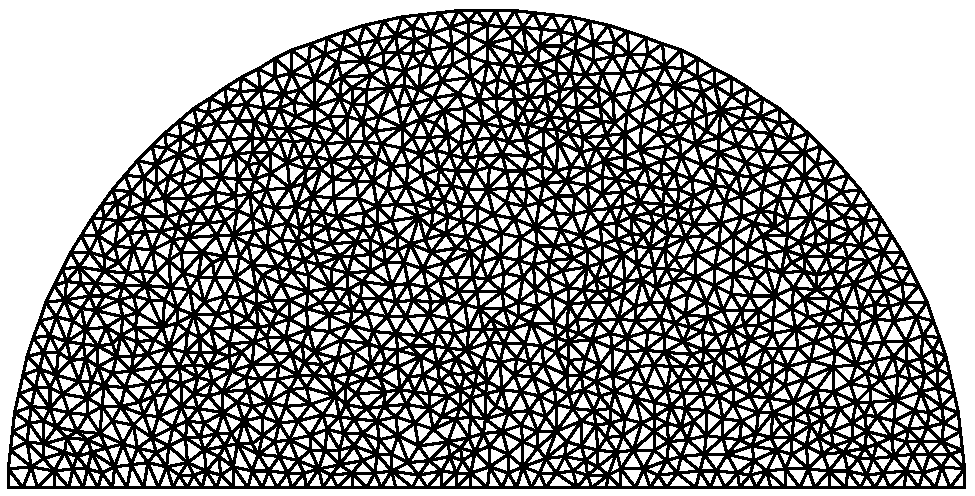
\includegraphics[width=\textwidth, keepaspectratio=1]{semicircle.pdf}
		\caption{Polkro\v zna cev.}
	\end{subfigure}
	\begin{subfigure}[b]{0.40\textwidth}
		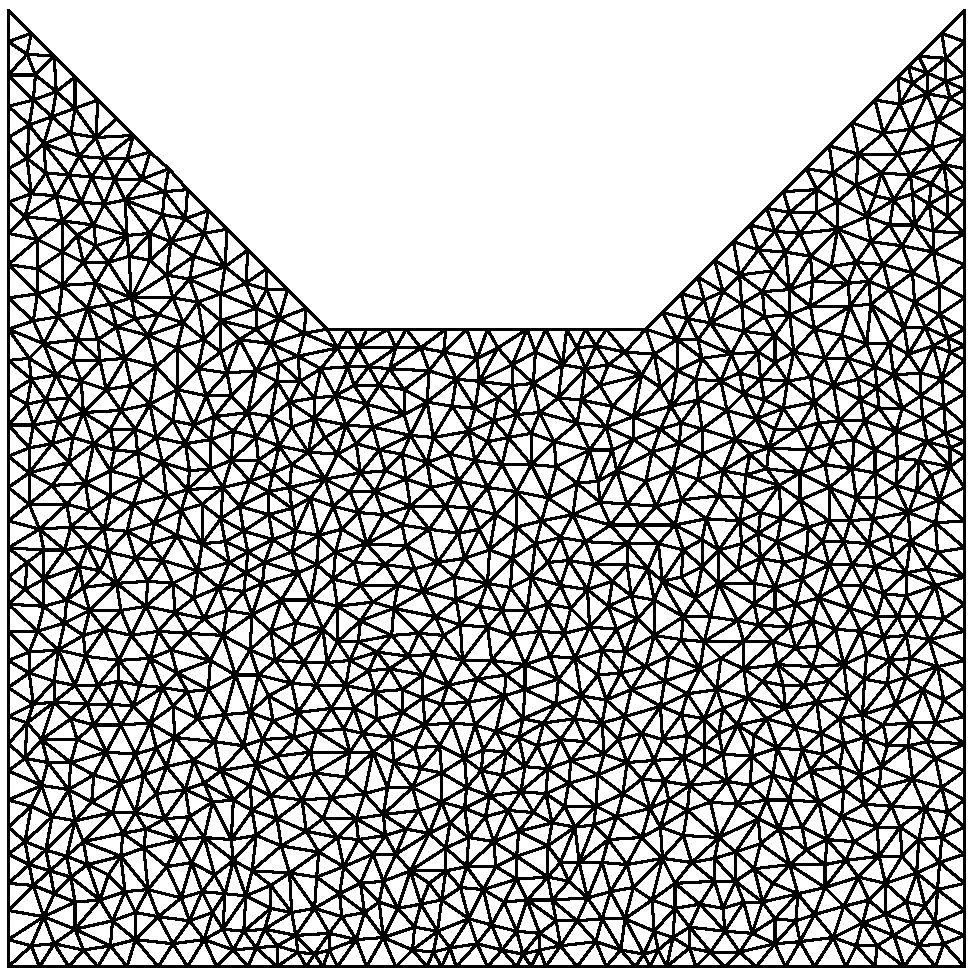
\includegraphics[width=\textwidth, keepaspectratio=1]{batman.pdf}
		\caption{Prirezana cev.}
	\end{subfigure}
	\caption{Delaunayeva triangulacija s programom \texttt{Triangle} za prvi in drugi del naloge.
		V obeh primerih je na\v sa mre\v za sestavljena iz $\sim 1000$ to\v ck.}
\end{figure}

\begin{thebibliography}{9}
	\bibitem{sirca}
		S. \v Sirca in M. Horvat,
		{\em Ra\v cunske metode za fizike},
		DMFA Zalo\v zni\v stvo,
		(2010)
	\bibitem{triangle}
		{\tt http://www.cs.cmu.edu/\~{}quake/triangle.html}
\end{thebibliography}

\end{document}
